

%Hi Tom, just some quick notes on the structure we discussed yesterday (4th Dec):
%
%- Aim to tell a chronological story with the progression of how CT/MRI scans have been consumed by professionals
%
%- The story in your first paragraph does not need to change. Following this there is some cut/paste to re-structure and group similar topics i.e. 2D and 3D.
%
%
%- then move onto all 2D examples - films to present data, and mention how they can be placed around the walls in a room to navigate them
% - Introduce computer displays to share the information i.e. all 2D
% - Discuss 3D on traditional displays
% - Move to immersive systems such as MR / VR...
% - Highlight the strength and the posibilities of immersive systems and perhaps xray vision as an example.
% - Then highlight the challenges: Misalignment, accuracy, followed by stating that this problem is the focus on your thesis

\chapter{Introduction} \label{Chap:Introduction}
% Explain what medical data is

%Tom perhaps consider adding something like this to the opening paragraph to make it clear your reserach is motivated my medical, but is also generic in its investigation to support other application areas. 
This thesis investigates visualisations that aim to understand and improve perception when using \gls{ost} augmented reality.
The topic area has been motivated by medical visualisations due to the need for data to be presented in a way that aligns intuitively with the user’s working area, ensuring that overlaid information is easy to interpret and supports natural understanding.
Although other application areas, such as manufacturing~\cite{Nguyen2016}, microbiological~\cite{Goodsell1989}, geological~\cite{Mathiesen2012, Liu2017}, and meteorological tasks~\cite{HibbardL.1986}, may also benefit from the perceptual support of the AR visualizations of this research.
Since the late 1980s, medical visualizations have provided healthcare professionals with a detailed and intuitive means of understanding complex anatomical structures, physiological processes, and pathological conditions within the human body. By translating intricate medical data into visual formats, medical visualizations aid in diagnosis, treatment planning, and patient education.
Medical visualizations can be derived from an extensive range of imaging techniques which can produce 3D datasets such as \gls{ct} scans, \gls{mri} scans, \gls{ultrasound}s, and \gls{xray}s as \gls{dicom} files.
These visualizations enable medical practitioners to assess and interpret the intricate spatial relationships between organs, tissues, and abnormalities accurately, facilitating more informed medical decision-making.
Moreover, these visualizations contribute to medical research by offering insights into disease progression, treatment effectiveness, and the development of innovative medical interventions.


Medical imaging technologies can utilize advanced photorealistic rendering derived from \gls{ct} and \gls{mri} scans, \gls{ai} methods for image understanding, and computational methods providing decision support to doctors. 
These technologies support medical professionals and help guide the planning and execution of procedures tailored to a patient's specific needs.
%\gls{ct} utilizes a series of X-ray beams that are reconstructed to produce a 3D image and are used to analyze bones, blood vessels, and tumors.
%\gls{mri} uses a strong magnetic field with a radio frequency to create a detailed image of the body by detecting the signals emitted as the corresponding hydrogen atoms realign. 
\gls{mri} images are typically used to view details with soft tissues but are also used to avoid the radiation caused by \gls{ct} scanners. 
\gls{ai}-based medical imaging is a newer technology used to view and provide ongoing analysis of tissue or indicate any immediate changes to the environment~\cite {Oren2020, Hosny2018}. 
%\gls{ai}-based medical imaging is created using sensor data that can be used to give new meaning to existing volumetric scans~\cite{Hosny2018, Bongratz2022}. 

\begin{figure}
    \centering
    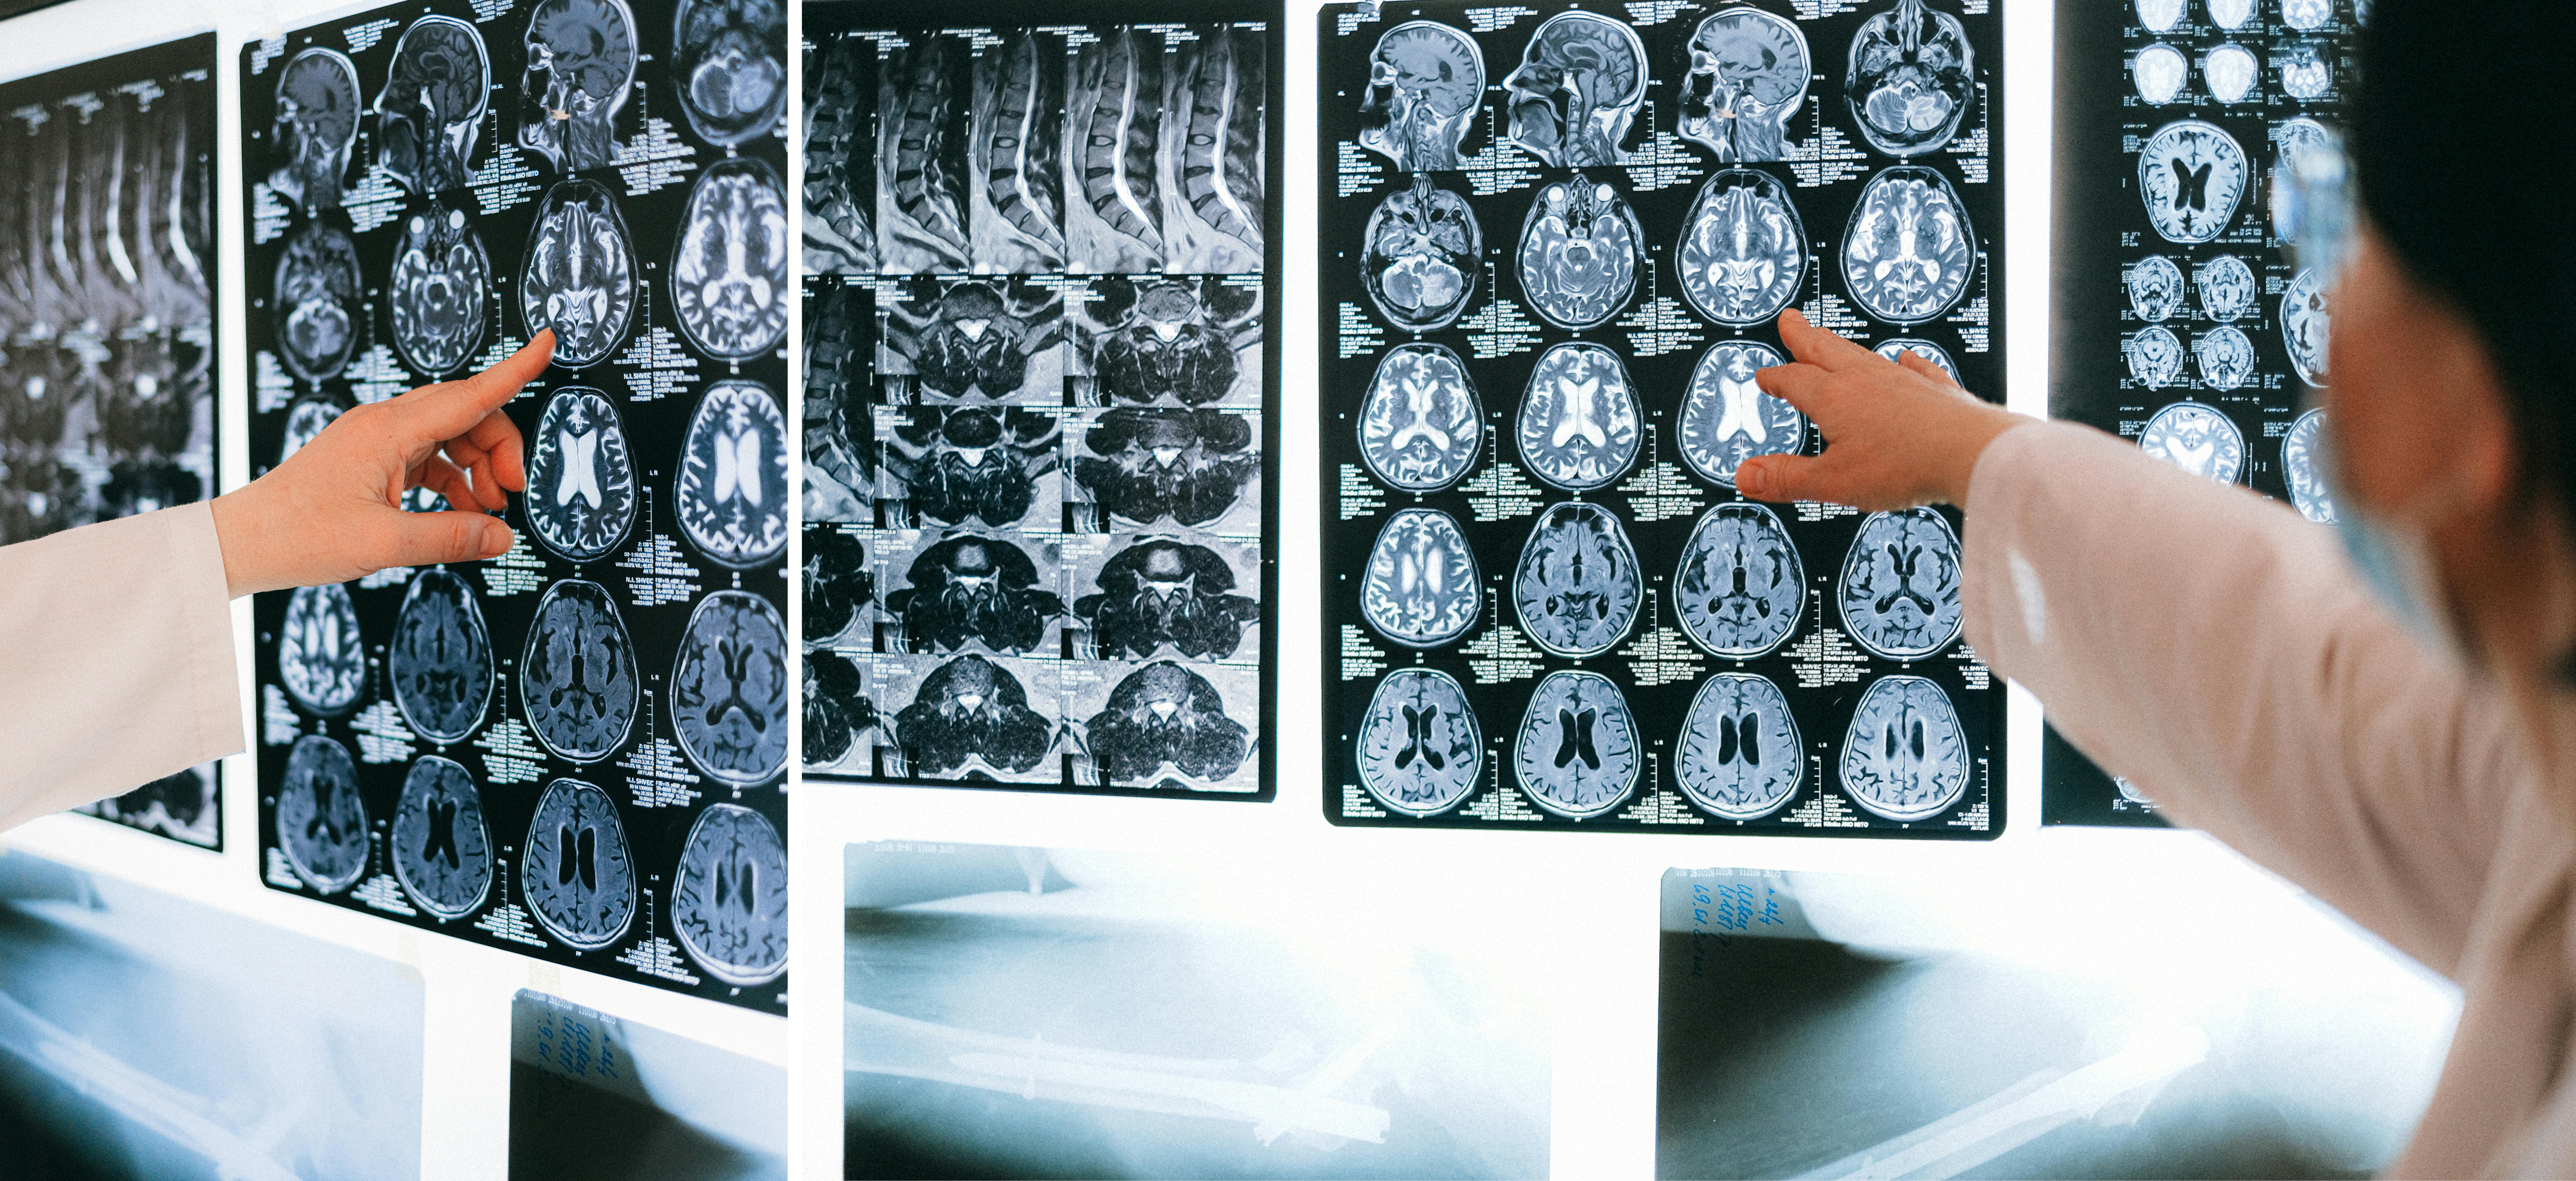
\includegraphics[width=\linewidth]{Chapter1/Images/pexels-shvetsa-MedicalFilms.png}
    \caption[Images of \gls{ct} and \gls{mri} films being utilized in a medical setting.]
    {
        Images of \gls{ct} and \gls{mri} films being utilized in a medical setting. 
        Anna Shvets took the photos shown here, which were licensed under a Creative Commons Attribuation licence~\footnotemark
    }
    \label{fig:MedicalFilms}
\end{figure}

% Jo Wants this to add limitations or current representations
%The display technology used to view tomographic data used in radiology and associated fields can impact the interpretation of the data.
Medical visualizations are commonly designed with 2D data in mind, as these tend to be viewed on desktop displays or tablets, or by more traditional display methods like placing films on light boxes and lit boards.  
2D visualizations require training in order to understand them, however experienced users can make more confident decisions with them due to understanding the structure of the human body~\cite{Jurgaitis2008}. 
Traditionally, \gls{mri} and \gls{ct} scans are printed onto transparent films and placed on adjustable light displays as shown in \autoref{fig:MedicalFilms}.~\footnotetext{\url{https://www.pexels.com/cs-cz/foto/ruka-doktor-ukazovani-lekar-4226264/}}
These adjustable light displays allow different scan slices to be visible in the film. 
These films are not easy to interpret for people without proper training.


Display technology employed to view tomographic data in radiology and related fields can significantly impact data interpretation.
Most medical visualizations displayed on a desktop typically represent 2D slices through the body.
%Since most monitors are limited to two dimensions of displaying data this has been known to be the preferred method as it most accurately utilizes the capabilities of the devices and interfaces~\cite{Mandalika2018}. 
Desktop and tablet interfaces will normally display this data in three different axes—one each for depth, width, or breadth—with an additional display presenting a 3D model for spatial awareness~\cite{Mandalika2018, Mast2019}.
This limitation may lead to solutions that only consider the primary axis.
%This limits the methodologies surgeons have to problem-solve in this space, leading to solutions that only consider the primary axis. 
This would allow surgeons to perform surgeries with more flexibility than they would currently be comfortable with~\cite{Dicken2005}.
%Tradional displays also suffer from the ambient and direct lighting conditions found in radiology reading rooms, coupled with the radiologist’s positioning of the display, can result in errors due to poorly calibrated displays and reflections. 
3D visualizations in some situations have been observed to be easier to understand, like identifying the distance between the operating area and high-risk areas or different methods to access the infected area~\cite{Dicken2005, Rieder2009, Cheung2021}.
This indicates that surgical planning could be further optimized and enhanced if 3D visualizations were displayed in a technically correct manner which is also contextually appropriate rendering and presentation. on their given displays and in the representative display environment. %\fixme{Explain what properly means}

\begin{figure}
    \centering
    \includegraphics[width=\columnwidth]{Chapter1/Images/CTandMRIScan.png}
    \caption[Two similar slices of different human heads.]
    {
        Two similar slices of different human heads: on the left, one a Magnetic Resonance Imaging (MRI) scan\footnotemark[1]; and on the right a Computed Tomography (CT) scan\footnotemark[2]. Both these images are licensed under a Creative Commons Attribution license.
    }
    \label{fig:CTAndMRI}
\end{figure}

%\fixme{Write a short paragraph about what CT and MRI scans and how they can be better used. }

% How is medical data used
% Explain what types what is a type of immersive technologies are

% Current research is investigating the use of 2D images in spatial environments. There are several challenges that have been identified including different pixel density of the screen's real estate and a mismatch between the expectations created by the spatial layout~\cite{St.John2001, Mandalika2018}.

On desktop displays, 2D visualizations can present shapes more clearly than 3D visualizations~\cite{Abbey2021, Zhou2022}. 
However, stereoscopic 3D displays (\gls{ar} and \gls{vr}) have been shown to represent 3D medical data as effectively as, or even better than, 2D visualizations~\cite{McIntire2012}.
Surgeons can navigate data from any angle, leading to a more intuitive presentation and greater precision~\cite{Ahlberg2007, Zhang2016a, Akpan2019}. 
These findings suggest that stereoscopic immersive \glspl{hmd} allow users to perceive 3D data naturally and intuitively~\cite{Vetter2002, Merino2018, Cecotti2021}. 
Most research on medical \gls{ar} has focused on 2D visualizations~\cite{Asadi2024}, likely due to the challenges that still need to be addressed in using immersive \gls{ar} devices for medical applications.


\footnotetext[1]{\url{https://www.flickr.com/photos/reighleblanc/3854685038}}
\footnotetext[2]{\url{https://pixabay.com/photos/head-magnetic-resonance-imaging-mrt-254863/}}
% What accommodations need to be taken for medicine
The use cases for \gls{ar} in medicine are inspiring, but there is a range of limitations that need to be addressed before \gls{ar} becomes common practice~\cite{Jha2021, Beams2022}. 
Firstly, medical practitioners may not risk losing sight of the real world~\cite{Beams2022}. 
This can happen by placing any camera-based or occlusive display over the user's eyes. 
This makes a \gls{vst} \gls{ar} \glspl{hmd} solution difficult because these systems have the potential to partially blind the user if they are unplugged or disconnected~\cite{Beams2022}.
Systems that are designed for robotic surgery that utilize a video-based surgery tend to use a robotic arm with inbuilt measures for removing any apparatus from the patient where a well-trained expert can aid the situation~\cite{Rosen2011}, preventing any issues that can occur from minor distortions of the input images. 
\gls{ar} \glspl{hmd} currently show a distorted view of reality, which can negatively influence depth perception and mislead users when performing precise interactions depending on the real world environment~\cite{Bichlmeier2007, Sielhorst2006}.
%Both Bichlmeier et al.~\cite{Bichlmeier2007} and Sielhorst et al.~\cite{Sielhorst2006} even when using techniques designed to minimise this impact that some unrealism existed. 
%\gls{ost} \gls{ar} does not have the limitations of having the user view the real world superimposed by the virtual world, but however, still has the limitations in regards to how the virtual world is viewed as compared to the real world. 
\gls{ost} \gls{ar} avoids the limitation of superimposing the real world with the virtual world. However, because this technology simply overlays information over the screen and covers the user's eyes, it still faces limitations in how the virtual world is perceived in comparison to the real world.

% Problems regarding  limitations of augmented reality
\gls{ost} \gls{ar} devices misrepresent users' depth perception compared to real-world vision, even under ideal conditions. 
These devices are not designed to fully align the virtual world with the user's perception, offering a view of the real world that is 'good enough' for most applications. 
Some \gls{ar} displays, such as \gls{ost} \gls{ar}, and sensors, like infrared cameras, struggle under bright lighting conditions. 
This causes inconsistent sensor readings and may reduce display visibility due to the \gls{ost} \gls{ar}'s shaded lens used to reflect light as a display~\cite{Geng2013, Xiong2021}. 
This shaded lens struggles to render transparent objects and can mandate a limited color gamut~\cite{Geng2013, Xiong2021}.
This lack of visibility and distortions caused by the display diminish users' spatial awareness of the \gls{ar} graphics~\cite{Jamiy2019, Rosales2019, Al-Kalbani2019, Armbruster2008}. 
These issues are less pronounced with mobile \gls{ar} and \gls{vst} \gls{ar} displays~\cite{Krevelen2010, Martin-Gomez2021}. 

\gls{ost} \gls{ar} devices all misrepresent their users' real depth perception compared to their real-world vision, even under ideal circumstances.
\gls{ar} devices are not designed to fully align the virtual world with the user's vision; they provide a good enough world viewpoint into the real world.
Some \gls{ar} displays (like \gls{ost} \gls{ar} displays) and sensors (such as infrared cameras) do not work under bright lighting conditions as they dim the colors shown in the display and introduce inconsistent sensor readings. 
Users' spatial awareness is also lessened when viewing graphics using \gls{ar}~\cite{Jamiy2019, Rosales2019, Al-Kalbani2019, Armbruster2008}. 
\gls{ost} \gls{ar} require a shaded lens to properly reflect light back at the users~\cite{Geng2013, Xiong2021}. 
These issues do not exist as much with mobile AR~\cite{Krevelen2010}. 
\gls{ost} \gls{ar} displays also have difficulties when rendering transparency due to their limited color gamut and how it is used to inform brightness~\cite{Geng2013, Xiong2021}.

This dissertation explores methods for visualizing spatial data to ensure AR-rendered graphics seamlessly integrate with physical-world objects, such as the human body. 
A key challenge for any AR system is accurately presenting objects located within or behind other objects~\cite{Bajura1992, Avery2009, Kalkofen2013, Parsons2021}.
To understand the data's location, humans typically need specific cues to perceive an object inside another, such as occlusion or a real-world metaphor like a hole. Without these cues, the data often appears to hover in front of the occluding object, giving the impression that it is positioned incorrectly.

% a 3D dataset or representation that can be visualized, often using techniques like volume rendering, which displays information throughout the 3D space
This research utilizes volume data as a medium, a 3D representation of space representing a set of samples from a given position relating to a given value in this area of the given voxel~\cite{Kaufman1999}.
volumes data allows this dissertation to move beyond traditional research by creating visualizations that utilize \gls{dvr}, allowing dynamic adjustments based on spatial and occlusion cues. 
This will enhance depth perception and improve integration with the physical environment. 
\gls{dvr} still allows for the same functionality as other graphical formats but provides new stereoscopic challenges that need to be overcome.
This dissertation also employs an off-the-shelf optical see-through (OST) AR device, the HoloLens 2~\footnote{\url{https://www.microsoft.com/en-au/hololens}}, which uses a lightly shaded lens and a waveform display to render images to ensure repeatability and consistency in testing these visualization techniques.

% % examples where controlling an ar device works well
% There are use cases of \gls{ar} where the aforementioned are not essential.
% Remotely controlling robotics using a Davinci system can be fine, since these systems are able to detect unsafe movements and have procedures in place~\cite{Rosen2011}. 
% However, when medical practitioners are using their hands or talking with patients, communicating these complex topics to their patients, they are required to see both the real world unobstructed and the virtual world where it is expected to be\cite{Marconi2017}.
% AR can provide spatial experiences that can be much more natural and intuitive than what is possible on desktop displays, for example, being able to move around and interact with objects in 3D space, but also provides the ability to see into 3D objects.

% % What is this thesis aiming to do
% This thesis explores how well volume data can be rendered in full volumes within solid real-world objects using an \gls{ost} \gls{ar} device.
% Ensuring objects appear where they are supposed to be, even if they are inside another real-world object.
% %While also ensuring that the distortion to depth perception, that is, by trying to remove this effect, is minimal.
% However, this thesis is not looking at testing the hardware. Instead, the research here uses off-the-shelf hardware of a HoloLens2~\footnote{\url{https://www.microsoft.com/en-au/hololens}}.
% Utilizing a lightly shaded lens with a waveform display to create images.
% %Many medical visualizations require the use of transparency.

\section{Motivations} \label{sec:IntroMotivations}
% Introduce this section 
% - Describe how what currently existed
% - Talk about what you did in Germany

% Talk about common visualizations in the field
Augmenting the real world using wearable devices (esp. \glspl{hmd}) is a promising field that has received much attention recently. Augmenting can take many forms, but seeing through or inside objects is particularly interesting in several domains.
It is common for immersive medical visualizations to present volume data as a 3D model so that it can be viewed from any direction. 
\glspl{hmd} allow for a natural way to view 3D data as users change their perspective by moving around the volume~\cite{Kasprzak2019, Pratt2018}.
\glspl{hmd} can be integrated with current systems to extend current working practices like cardiography~\cite{Kasprzak2019} and pathology~\cite{Hanna2018}. 

Hanna et al.~\cite{Hanna2018} looked into the potential of \gls{mr} within \gls{pathological} use cases, for example, enabling remote communication for autopsies for guidance and instruction using a 3D overlay and sharing scanned copies of specimens. 
\Glspl{pathologist}, like many medical professionals, are required to be able to keep a sterile environment. 
\gls{ar} \glspl{hmd}, like the HoloLens, utilize gesture commands that can keep an environment sterile and avoid with a keyboard and mouse which may contaminate the space.
This hands-free interaction is particularly beneficial in medical situations where sterility is paramount.

%They found that this type of work required the pathologist to communicate clearly to someone outside.
%This was generally done by touching something physical and infrared with the sterile nature of the work. 
%These communication protocols are the cause of several possible contamination issues. 
%By doing this, they gave people the ability to interact remotely within a completely sterile environment, allowing them to view information via the HoloLens display and use gestures without touching while keeping a sterilized environment.
%Allowing the pathologist to utilize these controls using gesture controls allowed the \gls{pathologist} to communicate to people outside of the sterile environment while seeing similar screens that did not affect their environment. 
%Users were able to annotate 3D objects and have other practitioners see the same scene as they are currently seeing, and they could mark up the virtual objects in it. 

\begin{figure}
    \centering
    \includegraphics[width=0.8\textwidth]{Chapter1/Images/HannaEtAlAutopsyHoloLensExample.PNG}
    \caption[A image of Hanna et al.'s~\cite{Hanna2018} sterile system for \glspl{pathologist}]{A image of Hanna et al.'s~\cite{Hanna2018} sterile system for \glspl{pathologist}. Used with permission from the College of American Pathologists}
    \label{fig:HannaEtAlAutopsyHoloLensExample}
\end{figure}

A wide range of medical visualizations fall outside the scope of volumetric data
but benefit from 3D medical visualizations by using \gls{gui} in conjunction with \gls{ar}. Endoscopies use a long flexible tube with a camera and light at one end to examine the inside of the body. Immersive approaches have created visualizations that hover above the body to provide medical practitioners with an indication of where inside of the body they are looking~\cite{Garcia-Vazquez2020}. Other visualizations have focused on guiding the practitioner with a Graphical User Interface (GUI) so they can either instruct people on what to expect in a given situation, like explaining to a nurse what tools she might be expected to use next~\cite{Unger2019}, or they could be used to try to communicate the angle and direction an incision should be performed using a 2D GUI projected on the area around the patient~\cite{Mewes2018}.
These applications could benefit from better in situ visualizations at a single point, providing a more natural interface and a more intuitive sense of data. 

% visualizations that aim to overlay information over a body
Research has explored overlaying a visualization for instructing a practitioner on using a syringe~\cite{Agten2018, Li2019a}.
Overlaying a \gls{mri} or \gls{ct} visualization has also been attempted on several occasions where it was found to to ensure that the medical practitioner can focus on what they are doing while observing the patient spontaneously and also the practitioner with annotations and instructions~\cite{Pratt2018, Si2018, Pratt2018, Blum2012}.
Visualizations can also educate the internal anatomy to less experienced practitioners or novices~\cite{Bajura1992}.

\subsection{Siemens Internship: Holographic Overlay System}

\begin{figure}
    \centering
    \includegraphics[width=0.8\textwidth]{Chapter1/Images/HolographicOverlaySystem.png}
    \caption{The Holographic Overlay system in use with a CT scanner.
    %\fixme{Miss aligned is incorrectly spelled}
    }
    \label{fig:HolographicOverlaySystem}
\end{figure}

% High-level overview and summary
Enabling medical practitioners to more intuitively understand their patients and helping to ease the education of medical data are intuitive benefits to companies specializing in creating machines to produce this data. 
%These benefits of overlaying began the foundation of an early internship I did at Siemens Forchheim, Germany, to understand what roadblocks still existed between using scan data overlaid over the patient's bodies. 
The benefits of data overlay formed the basis of an early internship I undertook at Siemens in Forchheim, Germany, where I explored the challenges still present in using scan data overlaid on patients' bodies.
At the commencement of this Ph.D. I was supported to travel to Siemens Forchheim, Bavaria, Germany, as an intern in the School of Health Sciences Digital Imaging \gls{ct} Research and Development Circulating Tumor Cells \gls{ai} department
%\gls{shs} \gls{di} \gls{ct} \gls{rd} \gls{ctc} \gls{ai} department. 
I was asked to create a system capable of overlaying the volumetric data from a CT scanner and calibrating it to the bed of a \gls{ct} scanner so it could be overlaid on the patient.
This allows radiologists to view the patient data as it is overlaid onto the patient and communicate with the current status of the \gls{ct} machine to track the patient.
%Moving the visualization as the \gls{ct} bed would also lift the patient up and down.

I was tasked with bringing the Booij et al.~\cite{Booij2019} research, which focused on a 2D interface that used a Kinect to collect a patient's anatomical data to aid radiologists in placing electrodes in the correct position on the patient's body utilizing a 3D reconstruction of the patient's body. 
The correct placement of electrodes on a patient’s body can be a difficult procedure to learn as it requires knowledge of where certain organs exist.
It is possible to determine where to place an electrode by evaluating the shape of the patient's body. 
An issue with the Booij et al.~\cite{Booij2019} system is that a 2D representation of a human is not always an accurate guide for varying body types since organs, muscles, and other body parts may be misplaced causing significantly different results~\cite{Kania2014,Hadjiantoni2021}.
By using a 3D \gls{hmd}, \gls{ar} display (HoloLens1), a 3D overlay could be made to instruct any operator of the \gls{ct} machine on how to use the system. 

After the CT scan had been completed, the system would replace the electrode guidance functionality with a visualization slice on a Sagittal Plane of the radiological data. 
This was replaced in the 3D system with an iso-surface or a \gls{dvr} visualization that was to be superimposed over the patient's body to better guide and inform the operator of the quality of the \gls{ct} scan.
This was aimed at lowering the required learning for \gls{ct} operators. 

% What was the system that was built
The gantry bed would need to be tracked, and its position known relative to the patient and the \gls{gantry} to provide the radiologist with instructions on where to place electrodes~\cite{Booij2019}. 
This allowed the volume to be visualized wherever the patient was, and it also provided flexibility for the operator to apply the electrodes. 
The final results of this system can be seen in \autoref{fig:HolographicOverlaySystem}.
The technical details of this system are described in more detail in \autoref{App:HolographicOverlaySystemDetails}.

Porting \gls{dvr} to a \gls{hmd} \gls{ar} display revealed more challenges than anticipated, primarily due to the high processing cost and the resulting visualization appearing slightly distorted in comparison to the surrounding environment.
This distortion was likely caused by the limited depth cues provided by \gls{ost} \gls{ar} displays, which made it difficult for users to determine the correct spatial position of virtual objects when physical objects were already present in the same location~\cite{Petri2018}.

One issue that was noted with the system was that the visualization was not dynamic and was only able to show a subset of a single range of the data before requiring to reload the information.
What was desired was the ability to view all of the data in a dynamic manner such as \gls{dvr}.  
For medical imaging, this capability is critical because important diagnostic features may not be confined to a single slice or range but distributed throughout the entire scan volume.
Being able to see the whole volume at once allows users to explore the data more intuitively and avoid missing relevant anatomical details or pathologies.
Particularly those with less specialized radiology training.

A prototype visualization of this can be seen in \autoref{fig:SiemensVolumeRendering} which presents a cube rendered with \gls{dvr}, showing the same inflated abdomen dataset as in \autoref{fig:HolographicOverlaySystem}, developed at Siemens Healthineers.
This visualization has several issues when viewed through an \gls{ar} display (Microsoft HoloLens), the visualization initially appeared to be in the correct spatial position. However, the stereoscopic properties of the \gls{hmd} made it evident that the visualization was rendered as a cube rather than a volumetric structure.
As a result, this method was ultimately excluded from the final version of the product.

\begin{figure}
    \centering
    \includegraphics[width=0.8\textwidth]{Chapter1/Images/VolumeRendering.png}
    \caption[This is a image of a cube rendered to show the same data shown in \autoref{fig:HolographicOverlaySystem} but using \gls{dvr}.]
    {
        This is a image of a cube rendered to show the same data of an inflated abdomen shown in \autoref{fig:HolographicOverlaySystem} but using \gls{dvr} which was developed at Siemens Healthineers.
    }
    \label{fig:SiemensVolumeRendering}
\end{figure}

% What was gained from this? 
\autoref{fig:HolographicOverlaySystem} depicts a challenge with the Holographic overlay system.
All of the visualizations that were supposed to be inside of the patient appeared smaller and outside of them. 
With enough time, users learned to orient themselves around this issue. 
This presentation of the data via \gls{ar} \gls{hmd} in this format seemed to cause more confusion about anatomy than simply displaying it on an external monitor or sitting above the patient.
%To repair this visual mismatch of visual data between the real and the augmented world, we propose to utilize X-ray vision. 

Overall, my Internship at Siemens highlighted that the current AR technologies were limited, including:
\begin{enumerate}
    \item When placing virtual objects behind or within real-world objects, there is a visual mismatch that occurs, causing the virtual object to appear misaligned. This issue is due to the difficulty in judging depth due to the lack of depth cues~\cite{Petri2018}.
    \item Sub-centimetre precision poses a general challenge for visualization and perception using \gls{mr} devices. The effect of \gls{ost} \gls{ar} visualizations on the user's depth perception requires further investigation.
    \item There currently exists no standard method to present frequently changing volumetric data inside an object.
    %\item Medical information is often displayed as a 3D space with continuously changing properties, not just a set of discrete objects. Current polygonal methods don't render such methods of data as a complete and whole manner.
    \item Medical information is often represented as volumetric data with continuously varying properties, rather than as discrete surface objects.
    Allowing for more direct contextual customization of the visualizations in real time paired with the ability to see the entire volume at once not just the given surfaces of a set range.
    Conventional polygonal rendering methods struggle to represent this type of data in a complete and integrated way.
\end{enumerate}



% % Talk about what was the current state of X-ray vision
% X-ray vision has been shown to repair this issue using virtual holes~\cite{Bajura1992}. 
% This solution still is not perfect. 
% While X-ray vision focused on medical situations, many of the solutions were designed to accommodate \gls{vst} display technology rather than \gls{ost} \glspl{hmd}, which would not have been practical in a medical situation~\cite{Wang2017a}.
% They all seemed to revolve around restricting the users' view of the data, making tasks like determining the \gls {ct} scan quality more challenging than needed.
% Another challenge was that most of the widely used solutions seemed to use image data or polygonal surface data. 
% I found that pre-processed rendering was too slow to allow for acceptable flexibility and was be accurate enough for the viewer. 


% % Why volume Rendering is so essential. 
% This dissertation is aimed at developing an understanding of how X-ray vision could be utilized and implemented into a system that utilized \gls{dvr}.
% \gls{dvr} is more flexible and allows for a clearer and more accurate view of the medical data, it can also be visulized at the same rate that the \gls{ct} scanner can produce images. 
% This would require not only fixing the technical issues that were found trying to implement \gls{dvr} into the system but also looking for a method of integrating x-ray visualizations into them while trying to overcome their inherent flaws for medical use. 
% %This inspired this research into how X-ray vision and X-ray visualizations work and how we can translate and validate them for medical purposes.
% Further, this research would require exploring how X-ray vision affects depth perception and also examining how it affects human behavior.
% %Then, studies will be performed to learn precisely how these effects work.
% %This study would need to evaluate a user's ability to utilize the visualization and investigate elements like participants' perceived cognitive load, how difficult they found the different effects to use, and how they behaved(speed and movement) regarding the various effects.



\section{Research Goal} \label{sec:IntroReserachGoal}
% % high-level view of all the challenges that need to be overcome.
% Today, medical practices are not employing Mixed Reality devices.
% This is due to a plethora of challenges.
% There are organizational issues that will prevent X-ray vision techniques adopted into the medical profession.
% These include funding, the possibility of the visualizations being distracting for the users, and challenges of how usable it really is usability, and an overall lack of training in using the tools~\cite{Jha2021}, while other issues stem from end-user resistance, and insurance matters~\cite{DaliliSaleh2022}. 
% Many of the issues preventing \gls{ar} from being adopted by my medicine will be solved over time through advances in other fields. 
% %Many of the issues regarding the usability \gls{ar} enabled x-ray vision will be resolved with time as technology becomes more ubiquitous. For example, UX design becomes more integrated in the design of \gls{ar} experiances~\cite{Jha2021}.
% Addionally technical issues such calibration~\cite{Xiong2021, Zhan2020}, limited color gambit~\cite{Xiong2021, Diaz-Barrancas2020}, heavy weight~\cite{Beams2022}, and comfort~\cite{Beams2022} can all be addressed by improving the hardware.

% talk on a high level about what this thesis aims to overcome
This research seeks to investigate the use of \gls{dvr} within physical objects when using \gls{ost} \gls{ar} \gls{hmd}s. 
The holographic overlay system displayed this data out of place.
\autoref{fig:DiagramX-rayVision} shows that the visualization is positioned correctly compared to the camera. However, because it is superimposed, it appears much larger and closer to the viewer. 
This was identified as a challenge to be addressed before systems become practical.
%Calibration would still be an issue, but since user perception seems to be the biggest issue, this would be our first step in ensuring that users perceive virtual objects to be in the locations where they are placed.
%Solutions for this are not well understood at this point; most solutions for X-ray vision are designed to work with \gls{vst} \gls{ar}, which is not well designed for high stress situations.

X-ray vision has been shown to repair this issue using virtual holes~\cite{Bajura1992}. 
However, this solution is not perfect. 
X-ray vision focused on medical situations, and many of the solutions were designed to accommodate \gls{vst} display technology rather than \gls{ost} \glspl{hmd}, which is not practical in a medical situation~\cite{Wang2017a}.
The solutions appeared to restrict the users' view of the data, making tasks like determining the \gls {ct} scan quality more challenging than needed.
The visualizations also utilized static geometry to generate the X-ray visualization while preventing the required level of flexibility.
%Another challenge was that most of the widely used solutions seemed to use image data or polygonal surface data. 
%I found that pre-processed rendering was too slow to allow for acceptable flexibility and was be accurate enough for the viewer. 

% \begin{figure}
%     \centering
%     \includegraphics[width=1\linewidth]{Chapter1//Images/X-rayVisionIllustration.jpg}
%     \caption{
%         An image comparing Superman's fictional X-ray Vision, which uses no real depth cues, with depth established cues found in Augmented Reality Enabled X-ray Vision. 
%         This image was illustrated by Brandly Richards for use in this thesis and is available under Creative Commons.
%     }
%     \label{fig:placeholder}
% \end{figure}


\begin{figure}
    \centering
    \includegraphics[width=1\linewidth]{Chapter1/Images/DiagramX-rayVisionMoreDetail.png}
    \caption{
        An example of where it is difficult to interpret depth due to the absence of depth cues. The circular object is a virtual object displayed against the wall in the next room. 
        \textbf{Left}) shows the room with no X-ray vision; \textbf{center}) shows the same room with X-ray vision enabled. However, the lack of depth cues makes it impossible to determine where the circular object in the next room is located. 
        \textbf{Right}) shows the same rooms as on the left, displayed using an isometric perspective to illustrate where the items are actually located.
    }
    \label{fig:DiagramX-rayVision}
\end{figure}

% is the motivation for investigating how DVR techniques can be developed for OST AR, particularly for X-ray vision.
The high-stress occupations found in medicine demand a level of predictability from the tools that they use. 
The influence on X-ray vision's ability to hinder perception has previously been tested~\cite{Santos2015}, but how it obscures spatial understanding is still unknown. 
%To start this investigation, it is imporant to learn how previously developed X-ray vision
There are also many unknowns about the ecological effects of X-ray vision, as most research in this area has mainly focused on perceptual tasks. 

% To address this, an experiment was conducted using these visualizations to ascertain the limits of human perception on \gls{ost} \gls{ar} by utilizing previously known X-ray visualizations.
% Adapting four different X-ray vision techniques that were designed to work on other devices to work on \gls{ost} \gls{ar} devices and by having participants perform a placement task, we were able to test out not only how these effects affected their depth perception but many other aspects of X-ray visualizations. 

% is the motivation for investigating visual cues that may aid in understanding spatial arrangement and relative depth perception.
\gls{dvr} itself has not been utilized on \gls{ost} \gls{ar} devices, despite having many applications in the medical domain alone. 
This, in turn, indicates there are a plethora of unknown consequences that may arise from its utility. 
% is the motivation for investigating the effect of visual cues on depth perception and the accuracy that can be achieved.
While creating X-ray visualizations that are designed to suit the \gls{ost} \gls{ar} display, it is important to note that these visualizations need to both suit the tasks they are required for and simultaneously function regardless of the use case. 
Ensuring these visualizations should suit the purposes where viewing \gls{dvr} information within the object itself is relevant, regardless if they are referring to manufacturing~\cite{Kanodia2005}, biological~\cite{Guo2012} or surgical tasks~\cite{Bajura1992}. 
These visualizations should be designed to allow users to view surfaces of any shape. 
X-ray visualizations should improve depth perception while allowing users to gain insight into the volume quickly.


% \begin{comment}
% \glspl{virt}
% \end{comment}

% A version of \gls{dvr} was developed that was designed to work within the limitations of \gls{dvr} was developed alongside three Volumetric Illustrative Rendering Techniques (VIRTs), which drew inspiration from 2D artistic effects to provide x-ray vision for \gls{dvr} objects viewed from an \gls{ost} \gls{ar}. 
% The impact that \glspl{virt} had on a person's ability to obtain information from the visualization as well as testing the effect of depth perception on the \glspl{virt}.


% % Pivit over to Volume rendering.
% Another large issue with X-ray vision in this field is that most \gls{X-ray Vision} techniques are designed to deal with solid and predictable surfaces like walls.
% Very few medical applications require their practitioners to look through walls. 
% People have paired X-ray vision with medical visualizations. However, they all focused on showcasing preprocessed data~\cite{Blum2012, Blum2012a, Kalkofen2007, Kalia2019}
% Walls are very different from human bodies; medical practitioners need to look through human bodies, which are much more curved and abstract than walls.
% \gls{mri} and \gls{ct} scans also don't tend to have a clearly defined surface. 
% Most items tend to get rapidly harder before they are dense enough to be solid. 
% To get around this, a method of performing X-ray vision can be flexible to work with abstract and curved surfaces that may not have clearly defined surfaces.


% % Talk about calibration issues
% Calibration of virtual objects anchored onto patients in medical science requires high precision (within 1mm)~\cite{Franz2014}.
% \gls{ar} struggles are not yet capable of this even in ideal settings with customized equipment~\cite{Swan2015}.
% Complications in the surgical environments caused by metallic medical equipment and distortions~\cite{Birkfellner1998} that can be triggered by user interactions~\cite{Ding2022, Soares2021} make this challenge much more difficult.
% The range of different \gls{ost} \gls{ar} \gls{hmd} displays also causes a prominent issue in the differences between depth perception evaluations range between 0.2cm and 2 cm~\cite{Swan2015, Rosales2019}.
% This distortion is even worse when you try to visualize an object behind a real-world object in AR~\cite{Bajura1992, Vishton1995}.

% % Talk about X-ray vision
% The field of X-ray vision has been looking at methods for placing virtual content beyond where it can easily be viewed~\cite{Bajura1992, Avery2008, Sandor2010}.
% Generally, when an object is rendered behind another object, it appears smaller but is perceived as being in front of the other object.
% When users move around the virtual space, the object will appear to move around or seem out of alignment.
% These issues, however, can be fixed when using X-ray vision~\cite{Bajura1992}. 

% % What is left to explore in X-ray vision
% The field of X-ray vision is very old in the field of Augmented Reality, having been researched for over 30 years~\cite{Bajura1992}.
% Many fields in this have been studied, ranging from depth perception to general usability~\cite{Bajura1992, Blum2012, Furmanski2002, Sandor2010, Otsuki2016, Tsuda2005, Zollmann2014}. 
% There are three main approaches to creating \gls{ar} enabled \gls{X-ray Vision} that can be used individually or together. 
% The most common is to render a texture over the surface that creates a degree of occlusion that the user can relate to~\cite{Kalkofen2007, Sandor2010, Otsuki2015}. 
% \gls{ar} X-ray Vision commonly archives highlights areas of interest in the real world and can manifest as geometric patterns calibrated to the physical world. 
% Another alternative is to create a visualization that conveys to the user the distance through objects such as a tunnel~\cite{Avery2009}. 
% The final option used is to show objects (virtual and physical) hidden in the physical world by rendering them as virtual objects~\cite{Bajura1992, Santos2015, Lerotic2007}.
% Unfortunately, there are still too many unknown factors to bring X-ray vision to the forefront.
% The field of X-ray vision does not have many ecological relevance user studies, meaning while depth is a well-explored area, the effects of spatial awareness especially have only seen little exploration~\cite{Li2016}, while precise spatial measures from X-ray vision have not been tested at all. 

% % Pivit over to Talk about issues regarding the headsets that have been worn
% Another issue is that \gls{X-ray Vision} research has tended to use \gls{vst} \gls{ar} devices, which, as mentioned at the start of this session, is poorly suited to medical purposes or other stressful occupations.
% This thesis aims to create the best quality X-ray vision possible for stressful occupations, allowing for \gls{ar} to stretch beyond our physical limitations of sight.
% To create the best quality \gls{X-ray Vision} effects, it is not only trying to build upon existing research but also using the lessons learned from this research to the field in question. 
% This thesis aims to find a method of X-ray vision for direct volumetric rendering using \gls{ost} \gls{ar} \gls{hmd} in a method that can be utilized in a stressful situation like surgery or medical diagnosis. 

The following factors motivate this research to focus on investigating:
\begin{itemize}
    \item How DVR techniques can be developed for OST AR, particularly for X-ray vision;
    \item If visual cues may aid in understanding spatial arrangement and relative depth perception;
    \item Observing the effects of visual cues and the accuracy that can be achieved on an \gls{ost} \gls{ar} \gls{hmd} display.
\end{itemize}

% % Since beginning this research several 
% This dissertation looks to find a form of X-ray vision that works on an \gls{ost} \gls{ar} device and can be utilized with \gls{dvr}.
% Leading to the creation of new \glspl{X-ray Visualization} for \gls{dvr} medical, microscopy, and any other application and verifying their effectiveness to use to test how they would function in real-world scenarios. 
% %This field of medical visualizations using \gls{ar} is becoming more topical as this field is moving on. 
% Since the beginning of this research, The field of x-ray vision for \gls{ost} \gls{ar} devices has flourished, showing that this is an incredibly relevant topic for today~\cite{MartinGomez2021, Fischer2020a, Gruenefeld2020, Guo2023, Fischer2023, Phillips2021}.
% This shows a growing demand for this research moving forward and further reinforcing my findings. 
% %My findings were backed up by the prior literature, which I used as a base for my research.
% %The initial phase involves reviewing previous work and then researching how well they interact within an ecologically relevant scenario. 

% \subsection{Direct Volume Rendering}
% % Why is this needed
% The holographic overlay system (Mentioned in \autoref{sec:IntroMotivations}) taught me how difficult to render in real-time based on when trying to visualize a large range of data. 
% Volume rendering requires no pre-processing allowing users to change the parameters they view in real-time and how they interact with it~\cite{Zhou2022}.
% This is very useful when working with medical data as it exists as a volume, and every \gls{voxel_g} can refer to a large range of densities dictated by the given \gls{hu_g}. 

% % A high-level overview of what DVR is
% \gls{dvr} uses simplified light physics algorithms to simulate how people could look through an object while retaining some semblance of reality.
% It does this by directly reading the volume data from memory and tracing the direction of light from the user's perspective.

% % 



% \subsection{Goals}
% % Why is X-ray vision important
% Users who navigate a complex object require adequate depth information regarding the position of objects to decide which actions to take.
% % Talking about limitations to superimposition
% The importance of accurate relative spatial perception can be seen in the work by Sielhorst et al.\cite{Sielhorst2006} and Pratt et al.\cite{Pratt2018}, who explored AR for 3D surgical guidance without using partial occlusion to aid in-depth perception. 
% %These works highlighted this technology's potential and current limitations in the field.
% Pratt et~al.~\cite{Pratt2018} mentioned the difficulties related to calibrating medical images superimposed on the patient while achieving correct spatial perception in the practitioner's view.
% Sielhorst et al.~\cite{Sielhorst2006} found that simulating a virtual window into the physical object was better than superimposing information on the patient's skin. 
% X-ray vision techniques were later integrated into this work by Bichlmeier et al.~\cite{Bichlmeier2007}.

% \textbf{Forming an understanding of what works and does not from previously used X-ray vision techniques}
% -
% To make this a reality we built a system that was capable of carrying over some highly published X-ray vision effects chosen via a systematic literature review \autoref{sec:X-rayBackGround}. We researched all of the X-ray vision effects from a VST AR headset over to an OST AR headset. 

% \textbf{Creating visualizations for Volumetric Data sets can be used for x-ray vision}
% -
% We take the lessons learned from this experiment and transition them to creating new visualizations for direct volume rendering.
% We then run two studies based on looking at these types of visualizations one to determine how well people can comprehend the data they are looking at and another one to test their improvements in depth perception. 

\section{Research Questions}
To address the research goals listed in \autoref{sec:IntroReserachGoal} focusing on creating \gls{X-ray Vision} methods for \gls{dvr}. 
This thesis will explore the following questions:

\begin{enumerate}[label=R.\arabic*]
    %\item Is there a difference in accuracy when placing a virtual object inside of a real world object when different X-ray visualization effects are used to describe the interaction of moving the virual object inside of the real object? (Chapter 3);
    \item How do X-ray visualization effects influence how accurately users can perceive the spatial alignment of a virtual object embedded within a real-world object? (Chapter 3);
    %\item How can Volumetric Illustrative Effects be adopted to become \gls{ost} \gls{ar} \gls{X-ray Vision} effects. (Chapter 4);
    \item Can \glspl{virt} aid a person’s comprehension of a volume when determining individual objects using direct volume rendering?  (Chapter 6);
    \item What is the minimum difference in depth that participants can reliably distinguish between volumetric objects, independent of any given \gls{virt}? (Chapter 7);
\end{enumerate}

\section{Contributions}
This thesis contributes the following:
\begin{enumerate}[label=C.\arabic*]
    \item A systematic literature review of \gls{X-ray Vision} describing the work to date. Presents an overview of the studies performed and an analysis of the use cases. (presented in Chapter 2, published in P.3);
    \item An algorithm that allows VST AR x-ray visualizations to be displayed on an OST AR device. (described in Chapter 3, published in P.4);
    \item Adapting X-ray techniques from \gls{vst} \gls{ar} to \gls{ost} \gls{ar}. (Presented in Chapter 4, published in P.6);
    \item A study comparing \gls{X-ray Vision} effects that had only previously been used on \gls{vst} \gls{ar} to be viewed on OST AR device. Showing that geometry-based \gls{X-ray Vision} techniques were better suited to OST AR devices (presented in Chapter 3, published in P.4);
    \item implementation of Volumetric \gls{X-ray Vision} utilizing Volumetric Illustrative Rendering Techniques (VIRTs). (described in Chapter 4, published in P.6);
    \item The Random Volume Generation System. A tool to randomly generate volumes that allow for controlled user studies in \gls{X-ray Vision}. (presented in Chapter 5, published in P.5); 
    \item A perception-based counting study to determine how well users could see the three VIRTs created. Findings show that different VIRTs could negatively and positively impact a user's ability to perceive accurately and determine what elements were in a volume. (presented in Chapter 6);
    \item A study to determine the different perceivable depth thresholds that the Hatching Stippling and Halo VIRTs can have between each other and a baseline condition by utilizing a 2FCA psychophysical study design. (presented in chapter 7);
\end{enumerate}

\section{List Of Publications} \label{section:Publications}
\begin{enumerate}[label=P.\arabic*]
    \item \textbf{Clarke, T. J.} (2021). Depth Perception using X-Ray Visualizations. 2021 IEEE International Symposium on Mixed and Augmented Reality Adjunct (ISMAR-Adjunct), 483–486. https://doi.org/10.1109/ISMAR-Adjunct54149.2021.00114
    \newline
    Contributed To: 
    \begin{itemize}
        \item Chapter 1;
    \end{itemize}
    
    \item Smith, R. T., \textbf{Clarke, T. J.}, Mayer, W., Cunningham, A., Matthews, B., \& Zucco, J. E. (2020). Mixed Reality Interaction and Presentation Techniques for Medical Visualisations. In P. M. Rea (Ed.), Biomedical Visualisation: Volume 8 (pp. 123–139). Springer International Publishing. https://doi.org/10.1007/$978-3-030-47483-6_7$
    \\
    Contributed To: 
    \begin{itemize}
        \item Chapter 1;
        \item Chapter 2;
    \end{itemize}

    \item \textbf{Clarke, T. J.}, Gwilt, I., Zucco, J., Mayer, W., and Smith, R T. (2024) Superpowers in the Metaverse: Augmented Reality Enabled X-Ray Vision in Immersive Environments. In Geroimenko V., Augmented and Virtual Reality in the Metaverse.
    \newline
    Contributed To: 
    \begin{itemize}
        \item Chapter 2;
    \end{itemize}

    \item \textbf{Clarke, T. J.}, Mayer, W., Zucco, J. E., Matthews, B. J., \& Smith, R. T. (2022). Adapting VST AR X-Ray Vision Techniques to OST AR. Proceedings - 2022 IEEE International Symposium on Mixed and Augmented Reality Adjunct, ISMAR-Adjunct 2022, 495–500. https://doi.org/10.1109/ISMAR-Adjunct57072.2022.00104
    \newline
    Contributed To: 
    \begin{itemize}
        \item Chapter 3;
    \end{itemize}

    \item \textbf{T. J. Clarke}, W. Mayer, J. E. Zucco and R. T. Smith, "Generating Pseudo Random Volumes for Volumetric Research," 2023 IEEE International Symposium on Mixed and Augmented Reality Adjunct (ISMAR-Adjunct), Sydney, Australia, 2023, pp. 266-270, doi: 10.1109/ISMAR-Adjunct60411.2023.00061.
    \newline
    Contributed To: 
    \begin{itemize}
        \item Chapter 4;
    \end{itemize}

    \item \textbf{T. J. Clarke}, W. Mayer, J. E. Zucco, A. Drogemuller and R. T. Smith, "Volumetric X-ray Vision Using Illustrative Visual Effects," 2023 IEEE International Symposium on Mixed and Augmented Reality Adjunct (ISMAR-Adjunct), Sydney, Australia, 2023, pp. 769-771, doi: 10.1109/ISMAR-Adjunct60411.2023.00168.
    \newline
    Contributed To: 
    \begin{itemize}
        \item Chapter 5;
    \end{itemize}

    % \item \textbf{T. J. Clarke}, B. J. Mattews, A. Drogemuller, W. Mayer, J. Zucco, R. T. Smith, "VIRTs: Volumetric Illustrative Rendering Techniques to Improve Individual Object Identification and Depth Understanding Using Ocular See Though Devices", ACM Transactions on Applied Perception.
    % \newline
    % Contributed To: 
    % \begin{itemize}
    %     \item Chapter 4;
    %     \item Chapter 6;
    %     \item Chapter 7;
    % \end{itemize}
    
\end{enumerate}

\section{Dissertation Structure}
Following this chapter is the literature review (Chapter 2), which will focus on all the related research done on \gls{mr} with a focus on medical applications, followed by a look into the research done on \gls{hci} regarding volumetric data and finished with a systematic literature review on \gls{X-ray Vision} covering all of the previous work done over the past 31 years in this field. 

% The results from the literature review were used to inform the next chapter's study design (in Chapter 3), which looks at a variety of popular \gls{X-ray Vision} effects that are designed to utilize a range of different \gls{ar} \gls{hmd}s by creating a system that allows \gls{vst} \gls{ar} techniques to be used on \gls{ost} \gls{ar} devices and then performed a spatial estimation task with them.

The results from the literature review were used to inform the study in Chapter 3, which looks at a variety of popular \gls{X-ray Vision} effects that are designed to utilize a range of different \gls{ar} \gls{hmd}s. 
To achieve this, a system was developed that allows \gls{vst} \gls{ar} techniques to be used on \gls{ost} \gls{ar} devices. 
This system was then used to perform a spatial estimation task, enabling an in-depth evaluation of how these effects function across different augmented reality hardware configurations.

Chapter 4 investigates the technical work involved in volume rendering and details the complexities involved in creating \gls{dvr} techniques for X-ray vision, concluding in the creation of the Volumetric Illustrative Rendering Techniques (VIRTs). 
This was followed by a modular method to create random volumes and details, the Random Volume Generation system. The Random Volume Generation system allows controlled studies to be conducted with volumes to access the VIRTs (described in Chapter 5).
The combination of the Random Volume Generation system and the VIRTs is then utilized in Chapter 6 to run a perception-based user study designed to determine how well a user can count regions within a volume. 
The chapter (Chapter 7) then took the VIRTs and tested the degree of depth thresholds users could reliably distinguish depth by utilizing a 2FCA psychophysical study.
The final chapter draws together the results and findings of this dissertation (Chapter 8).

